\subsubsection{Duration of Phase1}
First we will establish the number of pulls required in the first Phase so that we have a reasonable guarantee that the optimal arm does not get deleted at the end of the first Phase.
\begin{theorem}
The probability that the optimal arm $a^{*}$ will lie above $\dfrac{3}{4}\hat{\Delta}_{s}$ after $\dfrac{32}{9}\dfrac{ \log KT^{2}}{\epsilon}$ pulls in Phase1 is given by $\dfrac{1}{(|A|T^{2})^{\epsilon}}$, where  $0 < \epsilon\leq \min_{i\in A}{\Delta_{i}}$ and $\hat{\Delta}_{s}= \max\lbrace\hat{r_{i}}\rbrace-\min\lbrace\hat{r_{j}}\rbrace,i\neq j$
\end{theorem}
\begin{proof} \textbf{of theorem 1:}
From our assumption that the distributions are sub-Gaussian, we know that that after $s$ pulls,
\newline
$\mathbb{P} \lbrace\hat{r}^{*}-r^{*}  > \dfrac{3}{4}\hat{\Delta}_{s}\rbrace \leq \exp(\dfrac{{-s*(\dfrac{3}{4}\hat{\Delta}_{s})^{2}}}{2}) $
\newline
\newline
\hspace*{8em} $\leq \exp(-s*\dfrac{9}{32}\hat{\Delta}_{s}^{2}) $
\newline
\hspace*{8em} $\leq \exp(-\dfrac{\log |A|T^{2}}{\epsilon}\hat{\Delta}_{s}^{2})$, putting the value of $s=\dfrac{32}{9}*\dfrac{\log|A|T^{2}}{\epsilon}$
\newline
\hspace*{8em} $\leq \exp(-\dfrac{\log |A|T^{2}}{\epsilon}\epsilon^{2})$, since $\epsilon\leq \min_{i\in A}{\Delta_{i}}\leq \hat{\Delta}_{s} $  so that, $ \exp(-constant*\epsilon^{2}) > \exp(-constant*\hat{\Delta}_{s}^{2})$, where $constant > 0$
\newline
\newline
\hspace*{8em} $\leq \exp(-\epsilon\log |A|T^{2})$
\newline
\newline
\hspace*{8em} $\leq \dfrac{1}{(|A|T^{2})^{\epsilon}}$
\end{proof}

\subsubsection{Regret of Phase1}
\begin{theorem}
Let $\epsilon>0$ be a parameter such that $\dfrac{4}{9|A|}\Delta^{2}<\epsilon\leq \Delta$ and $\ell=\dfrac{32}{9}\dfrac{ \log |A|T^{2}}{\epsilon}$. The total regret suffered is $R_{\ell}\leq \max_{i\in A}{\Delta}_{i}\ell$, where $\Delta=\min_{i\in A}{\Delta_{i}}$
\end{theorem}
\begin{proof}\textbf{ of theorem 2:}
\cite{auer2002finite} proved that for UCB1, over a timestep $t$ the sample complexity of a sub-optimal arm is upper bounded by 
$\frac{8\log t}{\Delta_{i}^{2}} + 1 + \frac{\pi^{2}}{3}$. Let this be denoted by $s$. Now, let $\xi_{1}$ be the event such that $\sum_{i\in A} s\leq \ell$ for some $\epsilon>0$. Consequently, the regret is upper bounded by $\sum_{i \in A:r_{i}<r^{*}}\bigg(\frac{8\log \ell}{\Delta_{i}}\bigg) + \bigg(1 + \frac{\pi^{2}}{3}\sum_{i \in A}\Delta_{i}\bigg)$, as a sub-optimal arm might be pulled at most $s$ times if the duration of Phase1 is larger than $s|A|$. But we know that $\epsilon\leq\Delta$ and %$\sum_{i\in A}\bigg(\frac{8\log t}{\Delta_{i}^{2}} + 1 + \frac{\pi^{2}}{3}\bigg)>>\dfrac{32}{9}\dfrac{\log |A|T^{2}}{\epsilon}$. So, 
$\xi_{1}$ is possible only if,
\newline
\newline
\hspace*{8em}$\dfrac{32}{9}\dfrac{\log|A|T^{2}}{\epsilon}\geq \sum_{i\in A}\bigg(\dfrac{8\log t}{\Delta_{i}^{2}} + 1 + \dfrac{\pi^{2}}{3}\bigg)$
\newline
\newline
\hspace*{8em}$\Rightarrow \dfrac{32}{9}\dfrac{\log|A|T^{2}}{\epsilon}\geq \sum_{i\in A}\dfrac{8\log t}{\Delta_{i}^{2}} + |A|(1 + \dfrac{\pi^{2}}{3}) < |A|\dfrac{8\log t}{\Delta^{2}} + |A|(1 + \dfrac{\pi^{2}}{3})$
\newline
\newline
\hspace*{8em}$\Rightarrow \epsilon >  \dfrac{4}{9|A|}*\dfrac{\Delta^{2}\log|A|T^{2}}{\log t} + \dfrac{32}{9}\dfrac{\log|A|T^{2}}{|A|(1 + \dfrac{\pi^{2}}{3})}$ as $\Delta \leq \Delta_{i}, \forall i\in A$
\newline
At $t=|A|T^{2}$, $ \epsilon \leq \dfrac{4}{9|A|}\Delta^{2} + \dfrac{32}{9}\dfrac{\log|A|T^{2}}{|A|(1 + \frac{\pi^{2}}{3})}$
\newline
Ignoring the constant and bounding it loosely, we can say that, 
$\epsilon < \dfrac{4}{9|A|}\Delta^{2}$ results in Phase1 deciding the optimal arm and we need not go to the Phase 2. Also, at this point, the regret suffered will be close to UCB1 and more than UCB-Revisited.
\newline
\paragraph{}In another case, let $\xi_{2}$ be the event such that $\sum_{i\in A} s > \ell$ for some $\epsilon>0$.
In $\xi_{2}$, let sub-optimal arm $a_{1}$ is sampled more than optimal arm $a^{*}$. Let $a_{1}$ is sampled $s_{1}$ times and $a^{*}$ is sampled $s^{*}$ times and $s_{1}>>s^{*}$. Let $\Delta_{1}=r^{*}-r_{1}=\max_{i\in A}{\Delta}$ and in the worst possible case, $s_{1}-|A|+1=\ell$ (since $|A|$ arms are pulled atleast once in UCB1) and $s^{*}=1$. So the total regret suffered is $R_{\ell}\leq \max_{i\in A}{\Delta}_{i}\ell $ that is $R_{\ell}\leq \dfrac{32}{9}\dfrac{\max_{i\in A}{\Delta}_{i} \log KT^{2}}{\epsilon}$ .
\newline
\paragraph{}Somewhat a more better scenario is the third one, let $\xi_{3}$ be the event such that $\sum_{i\in A} s > \ell$ for some $\epsilon>0$.In $\xi_{3}$, let $a_{1}$ is sampled $s_{1}$ times and $a^{*}$ is sampled $s^{*}$ times and $0\leq |s_{1}-s^{*}|\leq\beta$, where $s_{1},s^{*},\beta\in \mathbb{N}$ and $\beta$ is a small integer. In $\xi_{3}$, let $\Delta_{1}=r^{*}-r_{1}=\max_{i\in A}{\Delta_{i}}$  and $s_{1}+s^{*}+|A|=\ell$. Hence $R'_{\ell}=max_{i\in A}{\Delta_{i}}s_{1}$. But, $s_{1}<\ell$ and $|s^{*}-s_{1}|\leq\beta $ so $R'_{\ell}<R_{\ell}$.
\newline
So the total regret suffered in Phase1 is $R_{\ell}\leq \dfrac{32}{9}\dfrac{ * \max_{i\in A}{\Delta}_{i} \log |A|T^{2}}{\epsilon}$, given $\dfrac{4}{9|A|}\Delta^{2}<\epsilon\leq \Delta$.
\end{proof}

\subsubsection{Arm Deletion}
\begin{theorem}
With an error probability of $e_{t}\leq \dfrac{2}{(\log |A|T^{2})^{1/4\epsilon}}$ 
%where $a=\dfrac{32}{9}\dfrac{\log KT^{2}}{\epsilon}$ is the duration of Phase1, 
we can delete an arm $a_{i}$ with $\bigg\lbrace\hat{r_{i}} + \sqrt{\dfrac{25}{32}\dfrac{\log{|A|T^{2}}}{\epsilon n_{i}}}\bigg\rbrace \leq \min_{i\in A}\hat{r}_{i}+\dfrac{1}{4} \hat{\Delta}_{s}$ after Phase1 where $\hat{\Delta}_{s}=\max_{j\in A}\hat{r_{j}} - \min_{i\in A}{\hat{r_{i}}}$, $i\neq j$, $\epsilon>0$ , $n_{i}$ is the number of times the arm $a_{i}$ was selected and $ n_{i} < \max_{j\in A:\hat{r}_{j}>\hat{r}_{i},\forall i\in A}\bigg\lceil\dfrac{{n_{j}}}{4}\bigg\rceil$, and $T$ is horizon.
\end{theorem}

\begin{proof}\textbf{ of theorem 3:}
The proof of this is given in \textbf{Appendix A}
\end{proof}


\section{Phase 2}

\subsection{Feedback from Phase1}
Let the number of times an arm $a_{i}$ is sampled till time $t$ (including Phase1) is $s_{i}$. After the initial exploration by Phase1, given that $\xi_{1}$ does not occur leave us with either $\xi_{2}$ or $\xi_{3}$. In such a scenario, in this section we will study the effect on arm deletion and early stopping condition.

\subsection{Proof:Phase 2}

\subsubsection{Deletion of Arms (First Condition)}
This arm deletion condition compares each arm $a_{i}$ with the optimal arm $a^{*}$. Here at each round $m$ it deletes any arm such that whenever $\tilde{\Delta}_{m}<\frac{\Delta_{i}}{2}$, arm $a_{i}$ gets deleted. This works best for cases when your arm set $A$ is dominated by large $\Delta_{i}, \forall i\in A$, because arms having large $\Delta_{i}$ gets deleted in the initial rounds. But this works very poorly if the $A$ is dominated by small $\Delta_{i}$ as it will wait till the later rounds to delete them, thereby increasing regret. 
\paragraph{}Here we will first prove the probability of deletion of a sub-optimal arm considering no feedback received from Phase1. After this we will prove that a feedback from Phase1 actually enhances the probability of deletion of arms.

\begin{theorem}
Without considering feedback from the  first phase, with a probability of $\bigg\lbrace 1-\dfrac{1}{2\psi(|A|)T\tilde{\Delta}_{m}^{2}}\bigg\rbrace$ a sub-optimal arm can be deleted in round m, where $\tilde{\Delta}_{m}$ is halved at the end of each round and $T$ is the horizon.
\end{theorem}

\begin{proof}\textbf{ of theorem 4:} Let at the end of $m$-th round, 
\newline
\hspace*{8em}$\hat{r}_{i}+c<\hat{r}_{j}-c$, where $\hat{r}_{j}$ is the arm with the highest average estimated reward in the $m$-th round.
\paragraph*{}So we will be considering lower bound of $\hat{r_{j}}$ and upper bound of $\hat{r_{i}}$. 
Let, in this round $\hat{r}_{j}=\hat{r}^{*}$.
Now, from Chernoff-Hoeffding bounds and considering independence of events,
\newline
\newline
\hspace*{8em}$\mathbb{P}\lbrace\hat{r}_{i} \geq r_{i} + c\rbrace \leq e^{-2(c)^{2}n_{m}}$
\newline 
\newline
Let, $c= \sqrt{\dfrac{log({4\psi(|A|)T\tilde{\Delta}_{m}^{2}})}{2\times n_{m}}}$
\newline Putting value of $c$ above,
\newline \hspace*{8em}$\mathbb{P} \lbrace  \hat{r}_{i} \geq r_{i} + c \rbrace \leq \dfrac{1}{4\psi(|A|)T\tilde{\Delta}_{m}^{2}}$
\newline Similarly, $\mathbb{P} \lbrace \hat{r}^{*} \leq r^{*} - c \rbrace\leq \dfrac{1}{4\psi(|A|)T\tilde{\Delta}_{m}^{2}}$
\newline
Summing the two up, the probability that sub-optimal arm not deleted in $m$-th round is $\dfrac{1}{2\psi(|A|)T\tilde{\Delta}_{m}^{2}}$
\end{proof}

\begin{corollary}
The number of times an arm $a_{i}$ is pulled in each round is $n_{m} = \bigg\lceil \dfrac{2log({T\psi(|A|)\tilde{\Delta}_{m}^{2}})}{\tilde{\Delta}_{m}^{2}} \bigg\rceil$ and this results in the condition $ \bigg\lbrace\hat{r_{i}}+\sqrt{\dfrac{log({T\psi(|A|)\tilde{\Delta}_{m}^{2}})}{2n_{m}}}\bigg\rbrace < max_{j\in B}\bigg\lbrace\hat{r_{j}}-\sqrt{\dfrac{log({T\psi(|A|)\tilde{\Delta}_{m}^{2}})}{2n_{m}}}\bigg\rbrace$ with probability $\bigg\lbrace 1-\dfrac{1}{2\psi(|A|)T\tilde{\Delta}_{m}^{2}}\bigg\rbrace$ where $B$ is the set of arms still not eliminated in the m-th round.
\end{corollary}

\begin{proof}\textbf{ of Corollary 5:}
The proof of this follows from \citep{auer2010ucb}. Let $c=\sqrt{\dfrac{log({T\psi(|A|)\tilde{\Delta}_{m}^{2}})}{2n_{m}}} $.
We know  that,
$\sqrt{\dfrac{log({T\psi(|A|)\tilde{\Delta}_{m}^{2}})}{2n_{m}}} = \sqrt{\dfrac{log({T\psi(|A|)\tilde{\Delta}_{m}^{2}}) * \tilde{\Delta}_{m}^{2}}{2 * 2log({T\psi(|A|)\tilde{\Delta}_{m}^{2}})} } = \dfrac{\tilde{\Delta}_{m}}{2}$, after putting the value of $n_{m}$. From this we know that, 
$c \leq \dfrac{\tilde{\Delta}_{m}}{2} =\tilde{\Delta}_{m+1} \leq \dfrac{\Delta_{i}}{4}$.
\newline
\hspace*{8em}$\hat{r}_{i} + c \leq \hat{r}_{i} + 2c $
\newline
\hspace*{11em}$< \hat{r}_{i} + 4c - 2c $
\newline
\hspace*{11em}$< \hat{r}_{i} + \Delta_{i} - 2c = r^{*} - 2c $
\newline
\hspace*{11em}$\leq r^{*} - c$
\newline
Thus, at the $m$-th round after pulling each arm $n_{m}$ number of times we get the elimination condition  $ \bigg\lbrace\hat{r_{i}}+\sqrt{\dfrac{log({T\psi(|A|)\tilde{\Delta}_{m}^{2}})}{2n_{m}}}\bigg\rbrace < max_{j\in B}\bigg\lbrace\hat{r_{j}}-\sqrt{\dfrac{log({T\psi(|A|)\tilde{\Delta}_{m}^{2}})}{2n_{m}}}\bigg\rbrace$ satisfied for some arm $a_{i}$ with the probability of $1 - \dfrac{1}{2\psi(|A|)T\tilde{\Delta}_{m}^{2}}$ as proved in Theorem 4. We have made this as a function of $|A|$, denoted by $\psi(|A|)$, such that $|\psi(|A|)|>1$ for any round $m$ and it should be a strictly monotonically decreasing function. This makes sure that at any round $m$, the value of $n_{m} = \bigg\lceil \dfrac{2log({T\psi(|A|)\tilde{\Delta}_{m}^{2}})}{\tilde{\Delta}_{m}^{2}}\bigg\rceil ,$ if $|\psi(|A|)|> 1$ is greater than $ \bigg\lceil \dfrac{2log({T\tilde{\Delta}_{m}^{2}})}{\tilde{\Delta}_{m}^{2}} \bigg\rceil$, thereby guaranteeing the above deletion condition of \textbf{Theorem 4}.
\end{proof}

From this we see that making the number of pulls in each round a function of $|A|$ increases the probability of deletion of arms when $|A|$ increases. This happens because now $n_{m}$ is a function of $|A|$ as $\psi(|A|)=|A|^{3/m}$ and thus the probability of deletion of arms in each round increases as long as $|\psi(|A|)|>1$. This is in contrast to \citep{auer2010ucb} where the number of pulls in each round are not dependent on $|A|$. But, the $\psi(|A|)$ should be strictly monotonically decreasing function with $|\psi(|A|)|>1$ at any round $m$, because if we make this function increase logarithmically or linearly, then the number of pulls increases more than quadratically and at later rounds the sub-optimal arms gets pulled substantially more than \citep{auer2010ucb} resulting in more regret. Infact, what we need is that $n_{m}$ should be atleast $n_{d}=\bigg\lceil \dfrac{2log({T\tilde{\Delta}_{m}^{2}})}{\tilde{\Delta}_{m}^{2}} \bigg\rceil$ and in the initial rounds pulling more number of times guarantees us better estimation of $\hat{r}_{i}$, but in the later rounds the number of pulls of each arm is already quite large and so a more tapered down function allows us to incur lesser regret but guarantees at least as much probability of arm elimination as pulling $n_{d}$ times. 

\paragraph*{} An initial exploration by Phase1 results in unequal pull of arms. The round-based scenario like in \citep{auer2010ucb} no longer exists as in that case, in each round, the arms are pulled an equal number of times. Here, we must first consider two cases. We incorporate the feedback from Phase1 into the average estimated reward and try to find whether the probability of deletion of arms increases or decreases. Let $\hat{r}_{i}$ be the estimated average payoff in Phase1 and $\hat{r'}_{i}$ be the estimated average payoff from Phase2 for $a_{i}, \forall i \in A$. We will consider 2 cases as mentioned in $\textbf{Theorem 6}$ below.

\begin{theorem}
Considering feedback from the first phase, with a probability of  $\bigg\lbrace 1-\dfrac{1}{4\psi(|A|)T\tilde{\Delta}_{m}^{2}} - \dfrac{1}{(4\psi(|A|)T\tilde{\Delta}_{m}^{2})^{1+\lambda}}\bigg\rbrace$,  we can delete a sub-optimal arm in round m, where $\tilde{\Delta}_{m}$ is halved at the end of each round  and $T$ is the horizon. 
\end{theorem}

Let, $c=\sqrt{\dfrac{log({4\psi(|A|)T\tilde{\Delta}_{m}^{2}})}{2n_{m}}}$, $c_{i}= \hat{r}_{i} + \sqrt{\dfrac{log({4\psi(|A|)T\tilde{\Delta}_{m}^{2}})}{2n_{m}}}$ and
$c^{*}= \hat{r}^{*} + \sqrt{\dfrac{log({4\psi(|A|)T\tilde{\Delta}_{m}^{2}})}{2n_{m}}}$.
\newline Here, $\hat{r}_{i}$ is the estimated average payoff in Phase1 and $\hat{r'}_{i}$ is the estimated average payoff from Phase2 for $a_{i}, \forall i \in A$.
%\newline Our approach in this proof will be to make the $\hat{r}_{i}$ from Phase1 a part of concentration interval as because $\hat{r}_{i}$ does not change after Phase1.

\begin{lemma}
If $\lambda c^{*}=c^{*}-c_{i}$ or $\lambda c_{i}= c_{i} - c^{*}$, then $\lambda$ value lies within the interval $(0, \dfrac{1}{\epsilon}]$
\end{lemma}

\begin{proof}\textbf{ of Lemma 7:}
Let, $c^{*}>c_{i}$
\newline
Now let, $\lambda c_{i}= c^{*}-c_{i}\Rightarrow \lambda c_{i} = \hat{r}^{*} -\hat{r}_{i}$
\newline
\hspace*{11em}$\Rightarrow \lambda = (\dfrac{\hat{r}^{*} - \hat{r}_{i}}{\hat{r}_{i}+c})$
\newline
Now, let $\hat{\Delta}_{1s}$ denote $\max_{i\in A}{\hat{r}_{i}}-\min_{i\in A}{\hat{r}_{j}}$, where $i\neq j$ in Phase1. So we can definitely say that if $a_{i}$ and $a^{*}$ survived Phase1 then they were definitely above $\min_{j\in A}r_{j}+\dfrac{1}{4}\hat{\Delta}_{1s}$. This also means that $|\hat{r}^{*} - \hat{r}_{i}|\leq \hat{\Delta}_{1s}$.
\newline 
\hspace*{11em}$\Rightarrow \lambda \leq (\dfrac{\hat{\Delta}_{1s}}{\hat{r}_{i}+c})$
\newline 
\hspace*{11em}$\Rightarrow \lambda < \hat{\Delta}_{1s}$
\newline 
\hspace*{11em}$\Rightarrow \lambda \leq \dfrac{1}{\epsilon}$, as $\hat{\Delta}_{1s}\geq \epsilon$
\newline 
%\hspace*{11em}$\Rightarrow -\dfrac{1}{4\epsilon}\leq\lambda\leq \dfrac{1}{4\epsilon}$
%\newline 
But, we know that $\epsilon> 0 $, hence $\lambda\in (0, \dfrac{1}{\epsilon}]$.
\newline
Similarly, for $c^{*} < c_{i}$ we can take, 
\newline
\hspace*{11em}$\lambda c^{*}= c_{i} - c^{*}\Rightarrow \lambda c^{*} = \hat{r}_{i} -\hat{r}^{*}$
\newline
\hspace*{11em}$\Rightarrow \lambda \leq \hat{\Delta}_{1s}\Rightarrow \lambda \leq \dfrac{1}{\epsilon}$, as $\hat{\Delta}_{1s}\geq \epsilon$
\newline 
Hence, for both cases we see that $\lambda\in (0, \dfrac{1}{\epsilon}]$
\end{proof}

\begin{proof}\textbf{ of theorem 6:}
\subsubsection*{\textbf{Case 1: $\hat{r}_{i} \leq \hat{r}^{*}$}}

Since, $\hat{r}_{i}< \hat{r}^{*}$ then $c_{i}<c^{*}$,
\newline
So in the $m$-th round let,
\newline 
\hspace*{8em}$\hat{r'}_{i}+c_{i}<\hat{r'}_{j}-c^{*}$, where $\hat{r'}_{j}$ is the arm with the highest average estimated reward in the $m$-th round. 
%\newline
%\hspace*{8em}$\Rightarrow \hat{r'}_{i}+c_{i}<\hat{r'}_{j}-c^{*} $
\newline
Let, in the $m$-th round $a_{j}=a^{*}$
\newline
\hspace*{8em}$\Rightarrow \hat{r'}_{i}+c_{i}<\hat{r'}^{*}-c^{*} $
\newline
Let, $c^{*}-c_{i}=\lambda c_{i}$, for some value of $\lambda $,
\newline
\hspace*{8em}$\Rightarrow \hat{r'}_{i} + c_{i}  < \hat{r'}^{*} - c_{i} - \lambda c_{i} $
\newline
\hspace*{8em}$\Rightarrow \hat{r'}_{i} + c_{i} < \hat{r'}^{*}-c_{i}( 1 + \lambda)  $
\newline
Now, from Chernoff-Hoeffding bounds and considering independence of events,
\newline 
\hspace*{8em}$\mathbb{P}\lbrace\hat{r'}_{i} \geq r'_{i} + c_{i}( 1 + \lambda)\rbrace \leq e^{-2(c_{i}(1+\lambda))^{2}n_{m}} \leq e^{-2(c(1+\lambda))^{2}n_{m}}$, as $c<c_{i}$ and $c,c_{i} > 0 $
\newline Putting value of $c$ above,
\newline\hspace*{8em} $\Rightarrow \mathbb{P} \lbrace  \hat{r'}_{i} \geq r'_{i} + c_{i}( 1 + \lambda) \rbrace \leq \dfrac{1}{(4\psi(|A|)T\tilde{\Delta}_{m}^{2})^{1+\lambda}}$
\newline Similarly, $\mathbb{P} \lbrace \hat{r'}^{*} \leq r'^{*} - c_{i} \rbrace\leq \dfrac{1}{4\psi(|A|)T\tilde{\Delta}_{m}^{2}}$
\newline
Summing the two up, the probability that sub-optimal arm not deleted in $m$-th round is $\dfrac{1}{4\psi(|A|)T\tilde{\Delta}_{m}^{2}} + \dfrac{1}{(4\psi(|A|)T\tilde{\Delta}_{m}^{2})^{1+\lambda}}$

\subsubsection*{\textbf{Case 2: $\hat{r}_{i} > \hat{r}^{*}$}}
Similiarly, since $\hat{r}_{i} > \hat{r}^{*}$ then $c_{i}>c^{*}$,
\newline
then let in $m$-th round,
\newline 
\hspace*{8em}$\hat{r'}_{i}+c_{i}<\hat{r'}_{j}-c^{*}$, where $\hat{r'}_{j}$ is the arm with the highest average estimated reward in the $m$-th round. 
\newline
Let, in the $m$-th round $a_{j}=a^{*}$
\newline
\hspace*{8em}$\Rightarrow \hat{r'}_{i}+c_{i}<\hat{r'}^{*}-c^{*} $
\newline
Let, $c_{i}-c^{*}=\lambda c^{*}$, for some value of $\lambda $
\newline
\hspace*{8em}$\Rightarrow \hat{r'}_{i} + c^{*} + \lambda c^{*} < \hat{r'}^{*}-c^{*} $
\newline
\hspace*{8em}$\Rightarrow \hat{r'}_{i} + c^{*}( 1 + \lambda) < \hat{r'}^{*}-c^{*} $
\newline
Now, from Chernoff-Hoeffding bounds and considering independence of events,
\newline 
$\mathbb{P}\lbrace\hat{r'}_{i} \geq r'_{i} + c^{*}( 1 + \lambda)\rbrace \leq e^{-2(c^{*}(1+\lambda))^{2}n_{m}}\leq e^{-2(c(1+\lambda))^{2}n_{m}}$, as $c<c^{*}$ and $c,c^{*} > 0 $
\newline Putting value of $c$ above,
\newline\hspace*{8em} $\Rightarrow \mathbb{P} \lbrace  \hat{r'}_{i} \geq r'_{i} + c^{*}( 1 + \lambda) \rbrace \leq \dfrac{1}{(4\psi(|A|)T\tilde{\Delta}_{m}^{2})^{1+\lambda}}$
\newline Similarly, $\mathbb{P} \lbrace \hat{r'}^{*} \leq r'^{*} - c^{*} \rbrace\leq \dfrac{1}{4\psi(|A|)T\tilde{\Delta}_{m}^{2}}$
\newline
Summing the two up, the probability that sub-optimal arm not deleted in m-th round is $\dfrac{1}{4\psi(|A|)T\tilde{\Delta}_{m}^{2}} + \dfrac{1}{(4\psi(|A|)T\tilde{\Delta}_{m}^{2})^{1+\lambda}}$
\newline
\paragraph*{}Now we know that $ 0 < \lambda \leq \dfrac{1}{\epsilon}$ and in case 1 and case 2, the probability of arm elimination increases as $\epsilon \rightarrow 0$  but $\dfrac{4}{9|A|}\Delta^{2}<\epsilon\leq \Delta$. %Generally a value of $\epsilon\approx \dfrac{\Delta}{2}$ suffices when $\Delta_{i}$ are small. 
This we can also see from the fact that as $\epsilon$ is smaller and smaller, the initial exploration (Phase1) is larger and larger and $\lambda$ also increases thereby decreasing the probability of arm not getting eliminated in the $m$-th round. The subsequent increase in probability compared to equal sampling of arms with no exploration is, 
\newline
$\bigg |\dfrac{1}{4|\psi(|A|)|T\tilde{\Delta}_{m}^{2}} + \dfrac{1}{(4\psi(|A|)T\tilde{\Delta}_{m}^{2})^{1+\lambda}} - \dfrac{2}{4\psi(|A|)T\tilde{\Delta}_{m}^{2}}\bigg | $ $\Rightarrow\bigg |\dfrac{1}{(4\psi(|A|)T\tilde{\Delta}_{m}^{2})^{1+\lambda}} - \dfrac{1}{4\psi(|A|)T\tilde{\Delta}_{m}^{2}}\bigg |$ 
\newline
\hspace*{18em}$\Rightarrow\bigg |\dfrac{1}{4\psi(|A|)T\tilde{\Delta}_{m}^{2}}( (4\psi(|A|)T\tilde{\Delta}_{m}^{2})^{-\lambda}-1)\bigg |$ for case1 and case2.


\end{proof}


\subsubsection{Deletion of Arms (Second Condition)}

One of the problems apparent in the first arm deletion condition which forced us to look at pivotal arm deletion condition is that when the $\Delta_{i}$ are very small then the regret suffered by UCB Revisited is massive. We know that when in $m$-th round $\tilde{\Delta}_{m} < \dfrac{\Delta_{i}}{2}$ the sub-optimal arm $a_{i}$ gets eliminated with a probability of $1-\dfrac{2}{4\psi(|A|)T\tilde{\Delta}_{m}^{2}}$. If not the arm gets over to the next $m+1$-th round. Now, when $\Delta_{i}$ is itself sufficiently small, only in later rounds the algorithm deletes the sub-optimal arm.
\paragraph*{}One way to alleviate this problem is to move the point of reference for deletion of arms close to poorly performing sub-optimal arms. This is achieved by the pivot arm denoted by $a_{p}$. In this method the algorithm first divides the arm set $A$ into quartiles based on the average estimated payoff $\hat{r}_{i}, \forall i \in A$. Then it selects a pivot arm (which may be sub-optimal) in the second and third quartile region which has the highest payoff in this region that is, it chooses an arm closest to the third quartile cutoff. If no such arm exists then it select the arm with lowest estimated payoff from the fourth quartile region (an arm closest to the third quartile cutoff lying in fourth quartile). Next any arms that doesn't suffice the necessary conditions are deleted. The novelty of this method is that for small $\Delta_{i}$, we no longer have to wait for the later rounds for arm elimination as the point of reference has been brought close to the poorly performing arms. We refer the reader to \textbf{Figure 1} for further illustrations.

\begin{figure}
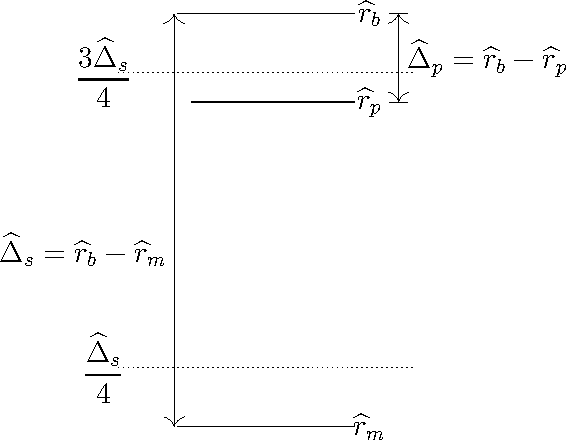
\includegraphics[scale=0.7]{img/diag1.pdf}
\caption{Pivotal Arm Deletion Case}
\end{figure}

\begin{theorem}
Without considering feedback from first phase, with a probability of $\bigg\lbrace 1-\dfrac{1}{2e^{(8/9)\epsilon}|A|T\tilde{\Delta}_{m}^{2}}\bigg\rbrace$ we can delete a sub-optimal arm in the m-th round satisfying the condition $\bigg\lbrace\hat{r}_{i}+\sqrt{\dfrac{log({4\psi(|A|)T\tilde{\Delta}_{m}^{2}})}{32n_{m}}} < \hat{r}_{p}-\sqrt{\dfrac{log({4\psi(|A|)T\tilde{\Delta}_{m}^{2}})}{32n_{m}}}\bigg\rbrace$, where $\hat{r}_{p}$ is the average estimated payoff from the pivot arm.
\end{theorem}

\begin{proof}\textbf{ of theorem 8:}
Let us start by considering the case:
\newline 
\hspace*{8em}$\hat{r}_{i}+c<\hat{r}_{p}-c$
\newline
So we will be considering the lower bound of $\hat{r_{p}}$ and upper bound of $\hat{r_{i}}$. So in the worst case $\hat{r_{p}}$ can be at a maximum distance of $\dfrac{3}{4}\hat{\Delta}_{s}$ from $\hat{r_{s}}$ 
\newline \hspace*{8em}$\Rightarrow \hat{r}_{i} + c <  \hat{r}_{s} - \dfrac{3}{4}\hat{\Delta}_{s} - c$
\newline \hspace*{8em}$\Rightarrow 4\hat{r_{i}} + 4c < 4\hat{r_{s}} - 3(\hat{r_{s}}-\hat{r_{m}}) - 4c$
\newline Let at the $m$-th round $\hat{r_{i}}=\hat{r_{m}}$(ie $a_{i}$ be any random arm which is below the $\dfrac{3}{4}\hat{\Delta}_{s}$ quartile)$,\hat{r_{s}}=\hat{r^{*}}$ (that is $a_{s}$ becomes the optimal arm in this round)
\newline \hspace*{8em}$\Rightarrow 4\hat{r_{i}} + 4c < 4\hat{r^{*}} - 3(\hat{r^{*}}-\hat{r_{i}}) - 4c$
\newline \hspace*{8em}$\Rightarrow \hat{r_{i}} + 4c < \hat{r^{*}} - 4c$
\newline
But, we have to condition this case of elimination on the probability that $r^{*}$ may lie any region above the $\hat{r}_{s}-\dfrac{3}{4}\hat{\Delta}_{s}$, where $\hat{r}_{s}$ is the arm with maximum payoff and the arm $a_{i}$ is lying below $\hat{r}_{m}+\dfrac{3}{4}\hat{\Delta}_{s}$ and $\hat{r}_{m}$ is the arm with minimum payoff.
\newline
\hspace*{8em}$\Rightarrow (\hat{r_{i}} + 4c)*\mathbb{P}\lbrace \hat{r}_{i} \leq \hat{r}_{m} + \dfrac{3}{4}\hat{\Delta}_{s}\rbrace < (\hat{r^{*}} - 4c)*\mathbb{P}\lbrace \hat{r^{*}} \geq \hat{r}_{s} - \dfrac{3}{4}\hat{\Delta}_{s} \rbrace$
\newline
Now, from Chernoff-Hoeffding bounds and considering independence of events,
\newline $\mathbb{P} \lbrace \hat{r'}_{i} \geq r_{i} + 4c \rbrace \leq e^{-2(4c)^{2}n_{b}}$
\newline 
Let, $c= \sqrt{\dfrac{log({4\psi(|A|)T\tilde{\Delta}_{m}^{2}})}{2\times 16n_{b}}}$
\newline Putting value of $c$ above,
\newline\hspace*{8em} $\Rightarrow \mathbb{P} \lbrace  \hat{r}_{i} \geq r_{i} + 4c \rbrace \leq \dfrac{1}{4\psi(|A|)T\tilde{\Delta}_{m}^{2}}$
\newline Similarly, $ \mathbb{P} \lbrace \hat{r}^{*} \leq r^{*} - 4c \rbrace \leq \dfrac{1}{4\psi(|A|)T\tilde{\Delta}_{m}^{2}}$
\newline
Again as in this round, $\hat{r}_{s} = \hat{r}^{*}$ we can trivially bound, 
\newline$\mathbb{P}\lbrace \hat{r^{*}} \leq \hat{r}_{s} - \dfrac{3}{4}\hat{\Delta}_{s} \rbrace\Rightarrow\mathbb{P}\lbrace \hat{r^{*}} \leq r^{*} - \dfrac{3}{4}\hat{\Delta}_{s} \rbrace \leq e^{-2*\dfrac{9}{16}\hat{\Delta}_{s}}$, 
\newline
\hspace*{11em}$\leq e^{-\dfrac{9}{8}\hat{\Delta}_{s}} \leq e^{-\dfrac{9}{8}\epsilon}$, as $\epsilon < \min_{i\in A}{\Delta_{i}} < \hat{\Delta}_{s}$
\newline
Similarly, $\mathbb{P}\lbrace \hat{r}_{i} \geq \hat{r}_{m} + \dfrac{3}{4}\hat{\Delta}_{s}\rbrace \leq e^{-\dfrac{9}{8}\epsilon}$, as $\hat{r}_{m}= \hat{r}_{i}$ in this round.
\newline
Summing everything up,
the regret that sub-optimal arm not deleted in a round is $\dfrac{1}{2e^{(9/8)\epsilon}\psi(|A|)T\tilde{\Delta}_{m}^{2}}$
\newline
\paragraph*{}Thus, we see from those proof that considering a pivot arm and doing arm elimination actually increases the arm elimination probability. This increase is dependent on the $\epsilon$ parameter itself as we conduct the initial exploration based on $\epsilon$.
\end{proof}

Again, we must consider the case of unequal pull of arms in this case as well because of the Phase1. 

\begin{theorem}
Considering feedback from the first phase, with a probability of  $\bigg\lbrace1-\dfrac{1}{4 e^{(9/8)\epsilon} \psi(|A|)T\tilde{\Delta}_{m}^{2}} - \dfrac{1}{(4 e^{(9/8)\epsilon} \psi(|A|)T\tilde{\Delta}_{m}^{2})^{1+\lambda}}\bigg\rbrace$ we can delete a sub-optimal arm in round $m$, where $\tilde{\Delta}_{m}$ is halved at the end of each round, $T$ is the horizon ,$A$ is the set of all arms.
\end{theorem}

\begin{proof}\textbf{ of theorem 9:}
The proof of this is given in \textbf{Appendix B}. It is proved in the same way as in \textbf{Theorem 6}.
\end{proof}


\subsubsection{Stopping condition}
%\begin{figure}
%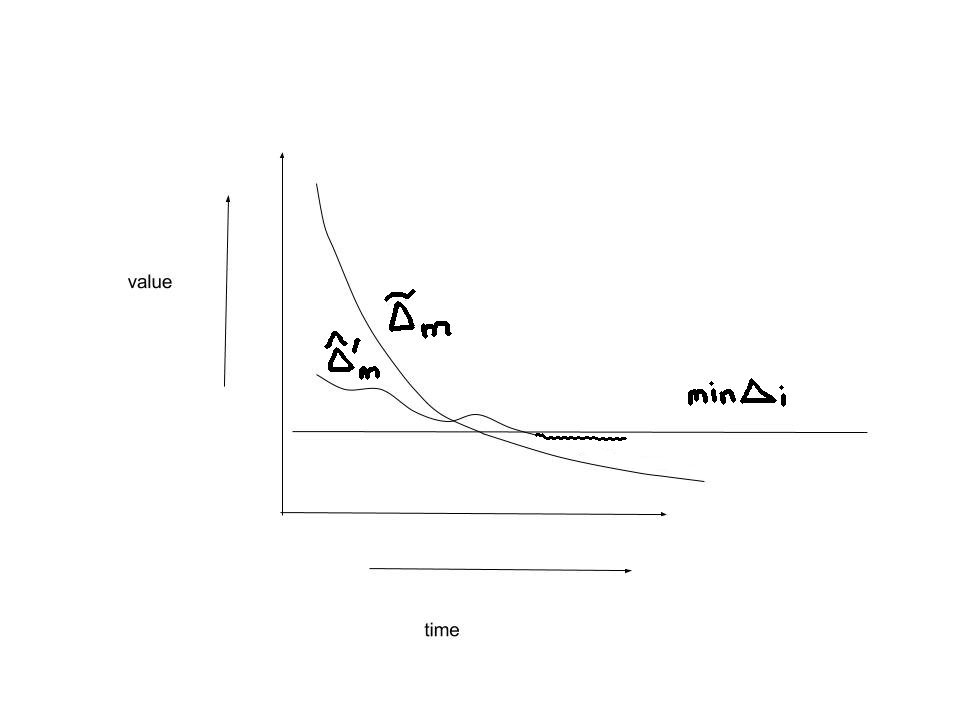
\includegraphics[scale=0.3]{img/final2_1.jpg}
%\end{figure}


In all the round based algorithms mentioned here \citep{auer2010ucb}, \citep{even2006action} (PAC -guarantees) or \citep{audibert2009exploration} (for budgeted bandits), the algorithm stops only when one  arm is left. But here as $\tilde{\Delta}_{m}$ gets halved after every round $m$, any sub-optimal arm is eliminated as soon as $\tilde{\Delta}_{m} < \dfrac{\Delta_{i}}{2}$, given the confidence interval holds as proved in \textbf{Corollary 5}. In such a situation if $\tilde{\Delta}_{m} < \min_{i\in A}\dfrac{{\Delta_{i}}}{2}$ there will be no arm to delete and we can output the optimal arm with certain probability. To early stop the rounds we can actually stop when $\tilde{\Delta}_{m} < \min_{i\in A}{\Delta_{i}}$ (that is one round before the final) and can output the optimal arm with some guarantee. The problem is we do not know the true $\min_{i\in A}{\Delta_{i}}$ but can only estimate it by $\hat{\Delta}'_{m}=\max\lbrace\hat{r_{i}}\rbrace-\max\lbrace\hat{r_{j}}\rbrace$, where $i\neq j $. Also just simply stopping when $\tilde{\Delta}_{m} < \hat{\Delta}'_{m}$ will not work because $\hat{\Delta}'_{m}$ will have to be sufficiently close to $\min_{i\in A}{\Delta_{i}}$ and stopping before will increase the error probability because of initial uncertainty over $\hat{\Delta}'_{m}$. But as the round proceeds we will get a better and better estimate of $\hat{\Delta}'_{m}$ whose value will be very close to $\min_{i\in A}{\Delta_{i}}$ in the later rounds. So to tide over the initial uncertainty as with all UCB based algorithms we add some confidence interval to it.

\begin{theorem}
With a probability of $\lbrace 1 - 2e^{-2(\dfrac{2^{m}}{2^{m/2}}c)^{2} n_{b}}\rbrace$ we can stop the rounds when, $\tilde{\Delta}_{m} + \sqrt{\dfrac{2^{-3/4} log({4\psi(|A|)T\tilde{\Delta}_{m}^{2}})}{n_{m}}} < \hat{\Delta}'_{m} - \sqrt{\dfrac{2^{-3/4} log({4\psi(|A|)T\tilde{\Delta}_{m}^{2}})}{n_{m}}}$ where $\hat{\Delta}'_{m}=\max\lbrace\hat{r_{i}}\rbrace-\max\lbrace\hat{r_{j}}\rbrace$ where $i\neq j $, $\tilde{\Delta}_{m}$ we half after every round and $m>1$.
\end{theorem}


\begin{proof}\textbf{ of theorem 10:}
The proof of this is given in \textbf{Appendix C}
\end{proof}

\begin{corollary}
Let $c=\sqrt{\dfrac{2^{-(1-\alpha^{2})/\alpha^{2}} log({4\psi(|A|)T\tilde{\Delta}_{m}^{2}})}{n_{m}}}$ be the confidence interval and $\alpha \geq 2$ be such a constant such that increasing its value results in faster convergence of $\tilde{\Delta}_{m} + \sqrt{\dfrac{2^{-(1-\alpha^{2})/\alpha^{2}} log({4\psi(|A|)T\tilde{\Delta}_{m}^{2}})}{n_{m}}} < \hat{\Delta}'_{m} - \sqrt{\dfrac{2^{-(1-\alpha^{2})/\alpha^{2}} log({4\psi(|A|)T\tilde{\Delta}_{m}^{2}})}{n_{m}}}$ where $\hat{\Delta}'_{m}=\max\lbrace\hat{r_{i}}\rbrace-\max\lbrace\hat{r_{j}}\rbrace$ where $i\neq j $, $\tilde{\Delta}_{m}$ is halved after every round and $m>1$.
\end{corollary}

\begin{proof}\textbf{ of Corollary 11:}
Let, in the $m$-th round, $c$ can also be written as $\sqrt{\dfrac{2^{\lbrace m/\alpha \rbrace^{2}} log({4\psi(|A|)T\tilde{\Delta}_{m}^{2}})}{2\times(2^{m})^2}n_{m}}$. It is quite apparent from the  proof  of \textbf{Theorem 10} that as $\alpha$ increases, the steeper is the fall of $c$, thereby increasing the probability of convergence before $\tilde{\Delta}_{m} < \min_{i\in A}\dfrac{{\Delta_{i}}}{2}$.
\end{proof}

\begin{corollary}
Considering the initial exploration in Phase1 with a probability of $\bigg\lbrace 1-\dfrac{2}{(4\psi(|A|)T\tilde{\Delta}_{m}^{2})^{1+\lambda}}\bigg\rbrace$, where $d=2^{m/2}$ the rounds can be stopped  when, $\tilde{\Delta}_{m} + \sqrt{\dfrac{2^{-3/4} log({4\psi(|A|)T\tilde{\Delta}_{m}^{2}})}{n_{m}}} < \hat{\Delta}'_{m} - \sqrt{\dfrac{2^{-3/4} log({4\psi(|A|)T\tilde{\Delta}_{m}^{2}})}{n_{m}}}$ where $\hat{\Delta}'_{m}=\max\lbrace\hat{r_{i}}\rbrace-\max\lbrace\hat{r_{j}}\rbrace$ where $i\neq j $, $\tilde{\Delta}_{m}$ is halved after every round and $m>1$.
\end{corollary}

\begin{proof}\textbf{ of Corollary 12:}
Now, $ 2e^{-2(\dfrac{2^{m}}{2^{m/2}}c)^{2} n_{b}} = \dfrac{1}{2\psi(|A|)T\tilde{\Delta}_{m}^{2}}$, after putting the value of $c$. Proceeding in the similar manner as in \textbf{Theorem 6} and \textbf{Lemma 7} we can prove after considering the 2 cases, and putting appropriate values of $\lambda$, that is,
\newline
let, $c_{i}= \hat{r}_{i} + dc_{i}$ and
$c^{*}= \hat{r}^{*} + dc^{*}$, where $d=\dfrac{2^{m}}{2^{m/2}}=2^{m/2}$ and $\hat{r}_{i}$ and $\hat{r}_{j}$ are the estimated average payoff from Phase1.
\newline
When, $\hat{r}_{i}>\hat{r}^{*}$, from Phase1, then
\newline
\hspace*{8em}$c^{*}\lambda=c_{i}-c^{*}\Rightarrow \lambda=\dfrac{\hat{r}_{i}-\hat{r}^{*}}{\hat{r}^{*}+dc^{*}}< \dfrac{\hat{r}_{i}-\hat{r}^{*}}{\hat{r}^{*}+c^{*}} $,as $d>1$
\newline
\paragraph*{}After this following the same way as in \textbf{Theorem 6} we can show that the probability of stopping in the $m$-th round is, $\bigg\lbrace 1-\dfrac{2}{(4\psi(|A|)T\tilde{\Delta}_{m}^{2})^{1+\lambda}}\bigg\rbrace$ and $\lambda\in (0,\dfrac{1}{\epsilon}]$.
\end{proof}

\section{Regret Bound Calculation}

\begin{theorem}
Combining Phase1 and Phase2 the total Regret over horizon T is $R_{T}\leq \dfrac{32}{9}\dfrac{ * \max_{i\in A}{\Delta}_{i} \log |A|T^{2}}{\epsilon} + \max_{i\in A}\bigg\lbrace\sum_{i\in A} (\dfrac{8}{\psi(|A|)\Delta_{i}} + \dfrac{8}{(\psi(|A|)\Delta_{i})(\psi(|A|)T\Delta_{i}^{2})^{(1/\epsilon)}}), \sum_{i\in A}(\dfrac{8}{ e^{(9/8)\epsilon} \psi(|A|)\Delta_{i}}$
\newline $+\dfrac{8}{(e^{(9/8)\epsilon}(\psi(|A|)\Delta_{i})(e^{(9/8)\epsilon} \psi(|A|)T\Delta_{i}^{2})^{(1/\epsilon)}})\bigg\rbrace + \sum_{i\in A}\bigg(\Delta_{i} + \dfrac{64log({T\psi(|A|)\Delta_{i}^{2}})}{\Delta_{i}}*\bigg(\dfrac{4}{\psi(|A|)T\Delta_{i}^{2}}\bigg)^{1+\frac{1}{\epsilon}}\bigg) + $\newline\newline$ e_{t} + \max_{i\in A}\Delta_{i}T$, 
where $\psi(|A|)$ is a monotonically decreasing function over $|A|$ and $|\psi(|A|)|>1$ for any round $m$, $0<\epsilon\leq \min_{i\in A}{\Delta_{i}}$, $e_{t}$ is the error bound and $T$ is the horizon.
\end{theorem}

\begin{proof}\textbf{ of theorem 12:}

\subsection{1st Phase}
The total regret suffered in Phase1 is $R_{\ell}\leq \dfrac{32}{9}\dfrac{ * \max_{i\in A}{\Delta}_{i} \log |A|T^{2}}{\epsilon}$, given $\dfrac{4}{9|A|}\Delta^{2}<\epsilon\leq \Delta$ where $\Delta=\min_{i\in A}{\Delta_{i}}$ (from section 7.1.2, \textbf{Theorem 2})
\subsection{2nd Phase}
For the second phase the regret will be calculated upon the stopping condition and arm deletion conditions. Let in the $m$-th round $\tilde{\Delta}_{m}<\dfrac{\Delta_{i}}{2}$ happens first time for some $a_{i}\in A$ and $A^{'}$ be the arm set containing arms still not eliminated till round $m$.

\subsubsection{\textbf{Case 1:}}
So, in the $m$-th round, the regret for not eliminating sub-optimal arms will be:
\newline
For the First Arm deletion condition the probability of arm not getting eliminated in $m$-th round is: $\dfrac{1}{4\psi(|A|)T\tilde{\Delta}_{m}^{2}} + \dfrac{1}{(4\psi(|A|)T\tilde{\Delta}_{m}^{2})^{1+\lambda}}$ from section 8.2.1, \textbf{Theorem 6}.
\newline
For the Second Arm(pivotal) deletion condition the probability of arm not getting eliminated in $m$-th round is: $\dfrac{1}{4 e^{(9/8)\epsilon} \psi(|A|)T\tilde{\Delta}_{m}^{2}} + \dfrac{1}{(4 e^{(9/8)\epsilon} \psi(|A|)T\tilde{\Delta}_{m}^{2})^{1+\lambda}}$ from section 8.2.2, \textbf{Theorem 8}.
\newline
\newline
Now, as in any round $m$, an arm $a_{i}$ gets deleted if it satisfies at least one of these arm deletion condition. If not that means both of these conditions failed to delete the arm $a_{i}$ and this condition is given by,
\newline 
$\max_{i\in A^{'}}\bigg\lbrace\sum_{i\in A^{'}}\bigg(\dfrac{1}{4\psi(|A|)T\tilde{\Delta}_{m}^{2}} + \dfrac{1}{(4\psi(|A|)T\tilde{\Delta}_{m}^{2})^{1+\lambda}}\bigg) ,\sum_{i\in A^{'}}\bigg(\dfrac{1}{4 e^{(9/8)\epsilon} \psi(|A|)T\tilde{\Delta}_{m}^{2}} + \dfrac{1}{(4 e^{(9/8)\epsilon} \psi(|A|)T\tilde{\Delta}_{m}^{2})^{1+\lambda}}\bigg)\bigg\rbrace$
\newline
\newline Summing up over all arms in $A^{'}$ and bounding the regret for each arm $a_{i}$ trivially by $T\Delta_{i}$,
\newline 
$\Rightarrow \max_{i\in A^{'}}\bigg\lbrace\sum_{i\in A^{'}} \bigg(\dfrac{T\Delta_{i}}{4\psi(|A|)T\tilde{\Delta}_{m}^{2}} + \dfrac{T\Delta_{i}}{(4\psi(|A|)T\tilde{\Delta}_{m}^{2})^{1+\lambda}}\bigg),\sum_{i\in A^{'}}\bigg(\dfrac{T\Delta_{i}}{4 e^{(9/8)\epsilon} \psi(|A|)T\tilde{\Delta}_{m}^{2}} $\newline\hspace*{20em}$+ \dfrac{T\Delta_{i}}{(4 e^{(9/8)\epsilon} \psi(|A|)T\tilde{\Delta}_{m}^{2})^{1+\lambda}}\bigg)\bigg\rbrace$
\newline
$\leq \max_{i\in A^{'}}\bigg\lbrace\sum_{i\in A^{'}} \bigg(\dfrac{1}{\psi(|A|)\Delta_{i}} + \dfrac{T\Delta_{i}}{(\psi(|A|)T\Delta_{i}^{2})^{1+\lambda}}\bigg) ,\sum_{i\in A^{'}}\bigg(\dfrac{1}{ e^{(9/8)\epsilon} \psi(|A|)\Delta_{i}} + \dfrac{T\Delta_{i}}{(e^{(9/8)\epsilon} \psi(|A|)T\Delta_{i}^{2})^{1+\lambda}}\bigg)\bigg\rbrace$
\newline
$\leq \max_{i\in A^{'}}\bigg\lbrace\sum_{i\in A^{'}} \bigg(\dfrac{8}{\psi(|A|)\Delta_{i}} + \dfrac{8}{(\psi(|A|)\Delta_{i})(\psi(|A|)T\Delta_{i}^{2})^{\lambda}}\bigg), $
\newline\hspace*{6em}
$\sum_{i\in A^{'}}\bigg(\dfrac{8}{ e^{(9/8)\epsilon} \psi(|A|)\Delta_{i}} + \dfrac{8}{(e^{(9/8)\epsilon}(\psi(|A|)\Delta_{i})(e^{(9/8)\epsilon} \psi(|A|)T\Delta_{i}^{2})^{\lambda}}\bigg)\bigg\rbrace$
\newline
$\leq \max_{i\in A^{'}}\bigg\lbrace\sum_{i\in A^{'}} \bigg(\dfrac{8}{\psi(|A|)\Delta_{i}} + \dfrac{8}{(\psi(|A|)\Delta_{i})(\psi(|A|)T\Delta_{i}^{2})^{1/\epsilon}}\bigg),$
\newline\hspace*{6em} $\sum_{i\in A^{'}}\bigg(\dfrac{8}{ e^{(9/8)\epsilon} \psi(|A|)\Delta_{i}} + \dfrac{8}{(e^{(9/8)\epsilon}(\psi(|A|)\Delta_{i})(e^{(9/8)\epsilon} \psi(|A|)T\Delta_{i}^{2})^{1/\epsilon}}\bigg)\bigg\rbrace$
\newline
\paragraph*{}Thus,we see that as $\epsilon$ decreases, the two terms $\dfrac{8}{(\psi(|A|)\Delta_{i})(\psi(|A|)T\Delta_{i}^{2})^{1/\epsilon}}$ and 
\newline $\dfrac{8}{(e^{(9/8)\epsilon}(\psi(|A|)\Delta_{i})(e^{(9/8)\epsilon} \psi(|A|)T\Delta_{i}^{2})^{1/\epsilon}}$ becomes negligible with a large $T$. %We have seen that generally $\epsilon\approx\dfrac{\Delta}{2}$ works fine in most of the cases.

\subsubsection{\textbf{Case 2:}}
Again, for any sub-optimal arm $a_{i}$ if not eliminated before this $m$-th round, is eliminated in this round or before or there is no sub-optimal arm in $A'$. In such a case the arm $a_{i}$ has to be played no less than,
\newline
\hspace*{8em}$n_{m,i}=\bigg\lceil \dfrac{2log({T\psi(|A|)\tilde{\Delta}_{m}^{2}})}{\tilde{\Delta}_{m}^{2}}\bigg\rceil \leq \bigg\lceil \dfrac{32log({T\psi(|A|)\dfrac{\Delta_{i}^{2}}{4}})}{\Delta_{i}^{2}}\bigg\rceil$,
\newline
Considering the early stopping condition, the probability of moving from one round to the next is given by $\dfrac{2}{(4\psi(|A|)T\tilde{\Delta}_{m}^{2})^{1+\lambda}}$, since the stopping condition is not fulfilled $(m-1)$th time, hence the total contribution of the $a_{i}$ arm which has survived till the $m$-th round is given by,
\newline
$n_{m,i}=\bigg\lceil \dfrac{2log({T\psi(|A|)\tilde{\Delta}_{m}^{2}})}{\tilde{\Delta}_{m}^{2}}*\dfrac{2}{(4\psi(|A|)T\tilde{\Delta}_{m}^{2})^{1+\lambda}}\bigg\rceil \leq \bigg\lceil \dfrac{32log({T\psi(|A|)\dfrac{\Delta_{i}^{2}}{4}})}{\Delta_{i}^{2}}*\dfrac{2.4^{1+\lambda}}{(\psi(|A|)T\Delta_{i}^{2})^{1+\lambda}}\bigg\rceil$
\newline
\hspace*{21em}$\leq \bigg\lceil \dfrac{64log({T\psi(|A|)\dfrac{\Delta_{i}^{2}}{4}})}{\Delta_{i}^{2}}*\dfrac{4^{1+\lambda}}{(\psi(|A|)T\Delta_{i}^{2})^{1+\lambda}}\bigg\rceil$
%\newline
\newline
\hspace*{21em}$\leq \bigg\lceil \dfrac{64log({T\psi(|A|)\dfrac{\Delta_{i}^{2}}{4}})}{\Delta_{i}^{2}}*\bigg(\dfrac{4}{(\psi(|A|)T\Delta_{i}^{2})}\bigg)^{(1+1/\epsilon)}\bigg\rceil$
\newline
\hspace*{21em}$\approx \bigg\lceil \dfrac{64log({T\psi(|A|)\Delta_{i}^{2}})}{\Delta_{i}^{2}}*\bigg(\dfrac{4}{(\psi(|A|)T\Delta_{i}^{2})}\bigg)^{(1+1/\epsilon)}\bigg\rceil$
\newline
The total contribution is,
$\sum_{i\in A'}\bigg(\Delta_{i}\bigg\lceil \dfrac{64log({T\psi(|A|)\Delta_{i}^{2}})}{\Delta_{i}^{2}}*\bigg(\dfrac{4}{(\psi(|A|)T\Delta_{i}^{2})}\bigg)^{(1+1/\epsilon)}\bigg\rceil\bigg)$
\newline
\hspace*{11em}$<\sum_{i\in A'}\bigg(\Delta_{i} + \dfrac{64log({T\psi(|A|)\Delta_{i}^{2}})}{\Delta_{i}}*\bigg(\dfrac{4}{\psi(|A|)T\Delta_{i}^{2}}\bigg)^{1+\frac{1}{\epsilon}}\bigg)$
\newline
\hspace*{11em}$<\sum_{i\in A'}\bigg(\Delta_{i} + \dfrac{64log({T\psi(|A|)\Delta_{i}^{2}})}{\Delta_{i}}*\bigg(\dfrac{4}{\psi(|A|)T\Delta_{i}^{2}}\bigg)^{1+\frac{1}{\epsilon}}\bigg)$
\newline
\paragraph*{}The error bound $e_{t}$ is proved in \textbf{Theorem 14}.
\newline
Thus, the total regret till round $m$ is given by,
$R_{T}\leq \dfrac{32}{9}\dfrac{ * \max_{i\in A}{\Delta}_{i} \log |A|T^{2}}{\epsilon} + \max\bigg\lbrace\sum_{i\in A^{'}} (\dfrac{8}{\psi(|A|)\Delta_{i}} + \dfrac{8}{(\psi(|A|)\Delta_{i})(\psi(|A|)T\Delta_{i}^{2})^{(1/\epsilon)}}), \sum_{i\in A^{'}}(\dfrac{8}{ e^{(9/8)\epsilon} \psi(|A|)\Delta_{i}} + \dfrac{8}{(e^{(9/8)\epsilon}(\psi(|A|)\Delta_{i})(e^{(9/8)\epsilon} \psi(|A|)T\Delta_{i}^{2})^{(1/\epsilon)}})\bigg\rbrace$
\newline + $\sum_{i\in A'}\bigg(\Delta_{i} + \dfrac{64log({T\psi(|A|)\Delta_{i}^{2}})}{\Delta_{i}}*\bigg(\dfrac{4}{\psi(|A|)T\Delta_{i}^{2}}\bigg)^{1+\frac{1}{\epsilon}}\bigg) + e_{t} + \max_{i\in A}\Delta_{i}T$.
\end{proof}

\section{Error Bound}
\begin{theorem}
Combining Phase1 and Phase2, the error bound is given by, $e_{t}\leq \dfrac{2T\max_{i\in A}{\Delta_{i}}}{(\log |A|T^{2})^{1/4\epsilon}} + \sum_{i\in A^{'}}\dfrac{16}{\psi(|A|)\Delta_{i}}+\sum_{i\in A^{''}\setminus A^{'}}\dfrac{16}{\psi(|A|)b}+
\sum_{i\in A^{'}}\dfrac{16}{e^{(9/8)\epsilon}\psi(|A|)\Delta_{i}}+\sum_{i\in A^{''}\setminus A^{'}}\dfrac{16}{e^{(9/8)\epsilon}\psi(|A|)b}$
\end{theorem}

\begin{proof} of \textbf{theorem 14}
\newline
The proof of this theorem is given in \textbf{Appendix D}
\end{proof}

Thus, we see from the total regret bound $R_{n}$ over horizon $T$ as proved in \textbf{Theorem 13}, the most significant term is $\sum_{i\in A^{'}}\bigg(\dfrac{64log({T\psi(|A|)\Delta_{i}^{2}})}{\Delta_{i}}*\bigg(\dfrac{4}{\psi(|A|)T\Delta_{i}^{2}}\bigg)^{1+\frac{1}{\epsilon}}\bigg)$. Comparing this to UCB-Revisited we see that we have achieved a significant improvement over the regret. Here, we must also consider that with a strong initial exploration we actually achieved a better result than UCB-Revisited as proved in \textbf{Theorem 6} and \textbf{Theorem 8}. But, $\epsilon$ must be guessed within a bounded range as established in \textbf{Theorem 2}.